% !Mode:: "TeX:UTF-8"
% !BIB program = bibtex
% !TEX program  = xelatex
\documentclass[UTF8]{ctexart} % 文档类型中文tex

% 设置页边距
\usepackage{geometry}
\geometry{a4paper,scale=0.9}

% 显示代码和结果
\usepackage{codeshow}

% tikz
\usepackage{tikz}
\usetikzlibrary{positioning}

% 文档信息
\title{tikz 画图}
\date{\today}

\tikzset{help lines/.style=very thin}
\tikzset{Karl's grid/.style={help lines, color=blue!50}}

\begin{document}

  \maketitle

  \section{简单图形}
  \subsection{直线}

  \begin{codeshow}
  \begin{tikzpicture}
    \draw (1,0) -- (0,0) -- (0,1);
  \end{tikzpicture}
  \end{codeshow}

  \begin{codeshow}
  \begin{tikzpicture}
    \draw (-1.5,0) -- (1.5,0);
    \draw (0,-1.5) -- (0,1.5);
  \end{tikzpicture}
  \end{codeshow}

\subsection{绘制曲线}

\begin{codeshow}
  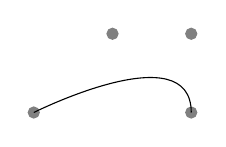
\begin{tikzpicture}
    \filldraw[gray] (0,0) circle [radius=2pt]
                    (1,1) circle [radius=2pt]
                    (2,1) circle [radius=2pt]
                    (2,0) circle [radius=2pt];
    \draw (0,0) .. controls (0,0) and (2,1) .. (2,0);

  \end{tikzpicture}
\end{codeshow}

可以通过这种方式画圆:
\begin{codeshow}
  \begin{tikzpicture}
    \draw (-1.5,0) -- (1.5,0);
    \draw (0,-1.5) -- (0,1.5);
    \draw (-1,0) .. controls (-1,0.555) and (-0.555,1) .. (0,1)
                 .. controls (0.555,1) and (1,0.555) ..(1,0);
  \end{tikzpicture}
\end{codeshow}

\subsection{绘制圆形}

\begin{codeshow}
  \tikz \draw (0,0) circle [radius=10pt];
\end{codeshow}

椭圆
\begin{codeshow}
  \tikz \draw (0,0) ellipse [x radius=10pt, y radius=5pt];
\end{codeshow}

接下来可以这样画圆形
\begin{codeshow}
  \begin{tikzpicture}
    \draw (-1.5,0) -- (1.5,0);
    \draw (0,-1.5) -- (0,1.5);
    \draw (0,0) circle [radius=1cm];
  \end{tikzpicture}
\end{codeshow}

\subsection{方形}
\begin{codeshow}
  \tikz \draw (-0.5,-0.5) rectangle (-1,-1);
\end{codeshow}

\subsection{绘制网格}
\begin{codeshow}
  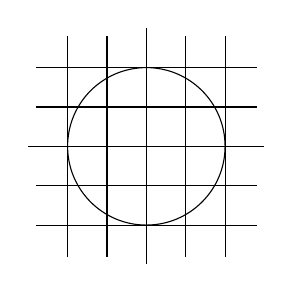
\begin{tikzpicture}
    \draw (-1.5,0) -- (1.5,0);
    \draw (0,-1.5) -- (0,1.5);
    \draw (0,0) circle [radius=1cm];
    \draw[step=.5cm] (-1.4,-1.4) grid (1.4, 1.4);
  \end{tikzpicture}
\end{codeshow}
然后将网格美化成灰色
\begin{codeshow}
  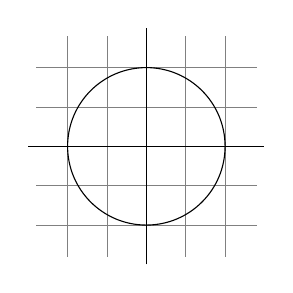
\begin{tikzpicture}
    \draw[step=.5cm, gray, very thin] (-1.4,-1.4) grid (1.4, 1.4);
    \draw (-1.5,0) -- (1.5,0);
    \draw (0,-1.5) -- (0,1.5);
    \draw (0,0) circle [radius=1cm];
  \end{tikzpicture}
\end{codeshow}

\subsection{增加风格}
提前设置风格会让代码更加灵活
\begin{codeshow}
  \tikzset{help lines/.style=very thin}
  \tikzset{Karl's grid/.style={help lines, color=blue!50}}
\end{codeshow}

之后可以这样画图
\begin{codeshow}
  \begin{tikzpicture}
    \draw[karl's grid] (0,0) grid(5,5);
  \end{tikzpicture}
\end{codeshow}

风格也可以作为tikzpicture 的参数
\begin{codeshow}
  \begin{tikzpicture}[
    my_grid/.style={help lines, color=#1!50},
    my_grid/.default=blue]

    \draw [my_grid] (0,0) grid (1.5,2);
    \draw [my_grid=red] (2,0) grid (3.5,2);

  \end{tikzpicture}
\end{codeshow}

\subsection{画弧}
\begin{codeshow}
  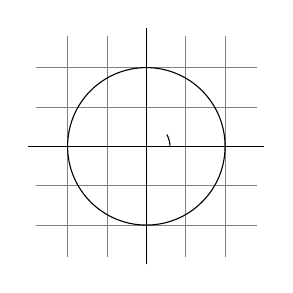
\begin{tikzpicture}
    \draw[step=.5cm, gray, very thin] (-1.4,-1.4) grid (1.4, 1.4);
    \draw (-1.5,0) -- (1.5,0);
    \draw (0,-1.5) -- (0,1.5);
    \draw (0,0) circle [radius=1cm];
    \draw (3mm, 0mm) arc [start angle=0, end angle=30, radius=3mm];
  \end{tikzpicture}
\end{codeshow}

可以用参数放大
\begin{codeshow}
  \begin{tikzpicture}[scale=2.5]
    \draw[step=.5cm, gray, very thin] (-1.4,-1.4) grid (1.4, 1.4);
    \draw (-1.5,0) -- (1.5,0);
    \draw (0,-1.5) -- (0,1.5);
    \draw (0,0) circle [radius=1cm];
    \draw (3mm, 0mm) arc [start angle=0, end angle=30, radius=3mm];
  \end{tikzpicture}
\end{codeshow}
也可以使用两个参数让圆弧变成椭圆弧线
\begin{codeshow}
  \tikz \draw (0mm, 0mm) arc [start angle=0, end angle=315, x radius=1.75cm, y radius=1cm];
\end{codeshow}

\subsection{剪辑弧线}
可以用\\clip命令只显示一部分, 在\\draw之前使用
\begin{codeshow}
  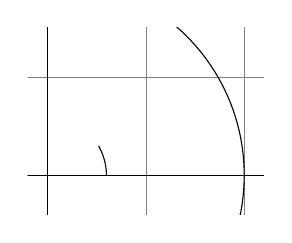
\begin{tikzpicture}[scale=2.5]
    \clip (-0.1, -0.2) rectangle (1.1,0.75);
    \draw[step=.5cm, gray, very thin] (-1.4,-1.4) grid (1.4, 1.4);
    \draw (-1.5,0) -- (1.5,0);
    \draw (0,-1.5) -- (0,1.5);
    \draw (0,0) circle [radius=1cm];
    \draw (3mm, 0mm) arc [start angle=0, end angle=30, radius=3mm];
  \end{tikzpicture}
\end{codeshow}

也可以绘制并裁剪
\begin{codeshow}
  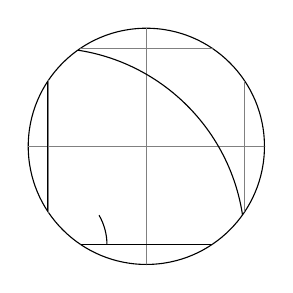
\begin{tikzpicture}[scale=2.5]
    \clip[draw] (0.5, 0.5) circle (.6cm);
    \draw[step=.5cm, gray, very thin] (-1.4,-1.4) grid (1.4, 1.4);
    \draw (-1.5,0) -- (1.5,0);
    \draw (0,-1.5) -- (0,1.5);
    \draw (0,0) circle [radius=1cm];
    \draw (3mm, 0mm) arc [start angle=0, end angle=30, radius=3mm];
  \end{tikzpicture}
\end{codeshow}

\subsection{抛物线和正弦线}

\begin{codeshow}
  \tikz \draw (0,0) rectangle (1,1) (0,0) parabola (1,1);
\end{codeshow}

\begin{codeshow}
  \tikz \draw [x=1pt,y=1pt](0,0) parabola bend (4,16) (6,12);
\end{codeshow}

也可以画正弦曲线
\begin{codeshow}
  A sine \tikz \draw [x=1ex,y=1ex] (0,0) sin (1.57,1); curve
\end{codeshow}

\subsubsection{绘图并填充}
\begin{codeshow}
  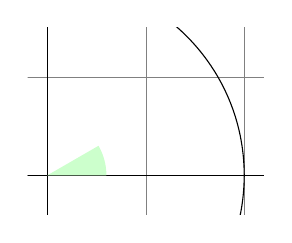
\begin{tikzpicture}[scale=2.5]
    \clip (-0.1,-0.2) rectangle (1.1,0.75);
    \draw[step=.5cm, gray, very thin] (-1.4,-1.4) grid (1.4, 1.4);
    \draw (-1.5,0) -- (1.5,0);
    \draw (0,-1.5) -- (0,1.5);
    \draw (0,0) circle [radius=1cm];
    \fill[green!20!white] (0, 0) -- (3mm, 0mm) arc [start angle=0, end angle=30, radius=3mm] -- cycle;
  \end{tikzpicture}
\end{codeshow}
颜色 green!20!white 是说 20\% 绿色和 80\% 混合.
--cycle 语句是路径闭合
\begin{codeshow}
  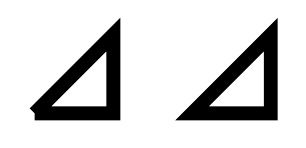
\begin{tikzpicture}[line width=5pt]
    \draw (0,0) -- (1,0) -- (1,1) -- (0,0);
    \draw (2,0) -- (3,0) -- (3,1) -- cycle;
  \end{tikzpicture}
\end{codeshow}

现在可以绘制并填充
\begin{codeshow}
  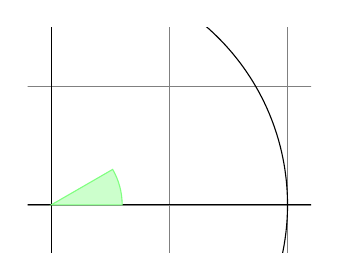
\begin{tikzpicture}[scale=3]
    \clip (-0.1,-0.2) rectangle (1.1,0.75);
    \draw[step=.5cm, gray, very thin] (-1.4,-1.4) grid (1.4, 1.4);
    \draw (-1.5,0) -- (1.5,0);
    \draw (0,-1.5) -- (0,1.5);
    \draw (0,0) circle [radius=1cm];
    \filldraw[fill=green!20!white, draw=green!50!white] (0, 0) -- (3mm, 0mm) arc [start angle=0, end angle=30, radius=3mm] -- cycle;
  \end{tikzpicture}
\end{codeshow}

\end{document}
